\section*{Redes con patrón (\emph{blazing})}

\item (*)
\begin{enumerate}
\item Escriba la función transmisión para una red de rendijas de ancho $b$ y período $d$.
\item Idem (a) para una red formada por prismas delgados de alto $b$ y base $a$, con índice de refracción $n$, y separados por tramos obstruidos de alto $d-b$ (ver figura). 
\end{enumerate}
\begin{figure}[h]
	\centering{}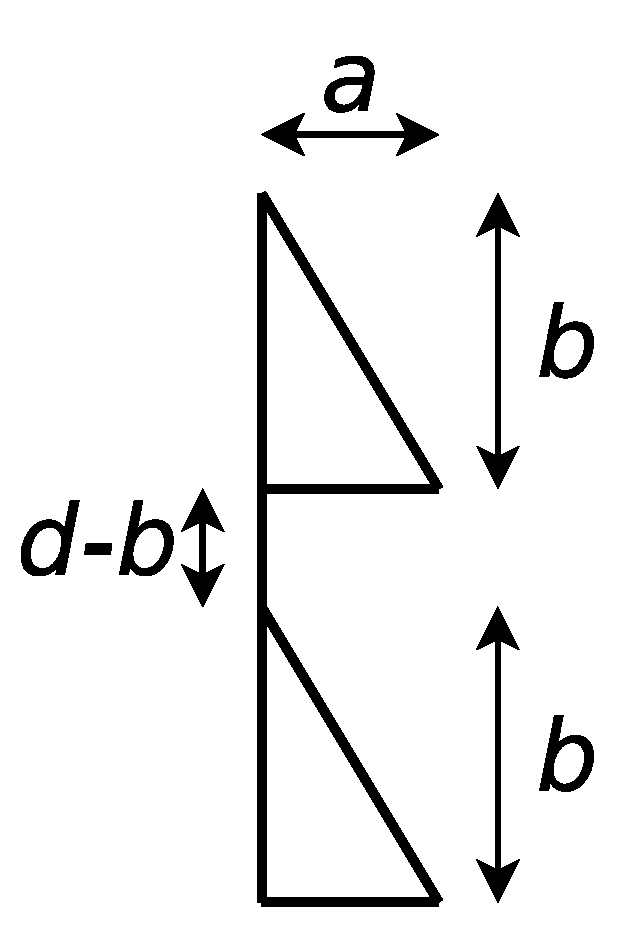
\includegraphics[clip,scale=0.3]{ej5-44}
\end{figure}



%\item (*)
%\begin{enumerate}
%	\item Hallar la distribución de intensidades sobre la pantalla para la red de transmisión descripta en el problema anterior.
%	La luz incide con un ángulo arbitrario sobre la red.
%	\item Comparar la distribución obtenida con la de una red de transmisión de $N$ rendijas de ancho $b$ y período $d$. ¿En qué se diferencian? 
%\end{enumerate}



\item (*) Se tiene una red de difracción de $N$ períodos como se muestra en la figura.
Se trata de una distribución de pares de prismas delgados de índices $n_{1}$, y $n_{2}$ y ángulos $\delta_{1}$ y $\delta_{2}$, respectivamente (ver figura).
Se la ilumina en forma normal.
Suponiendo que la teoría fuese exacta:
\begin{figure}[h]
	\centering{}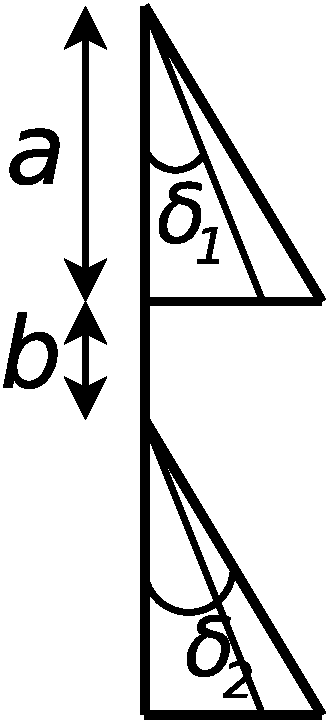
\includegraphics[clip,scale=0.3]{ej5-46}
\end{figure}
\begin{enumerate}
	\item Halle la intensidad en la pantalla como función del ángulo $\theta$. 
	\item Elija parámetros de la red ($n_{1}$, $n_{2}$, $\delta_{1}$, $\delta_{2}$, $a$, $b$, $N$), para los cuales se intensifique el orden ($-2$) para una longitud de onda incidente de 5000 Å, y para que se puedan resolver las longitudes de onda de 5000 Å y 5001 Å, en dicho orden. 
\end{enumerate}


\item (*) Una red de transmisión de ancho 2 cm está formada por 50 prismas delgados.
Sabiendo que intensifica el segundo orden de interferencia, para $\lambda=5000$ Å calcule: 
\begin{enumerate}
	\item El ángulo de \emph{blazing}. 
	\item La posición angular del orden intensificado y de la imagen geométrica. 
	\item Discuta, en este caso, qué sucede con los otros órdenes de interferencia para la longitud de onda $\lambda$ dada.
	\item Calcule el poder resolvente para el segundo orden. 
\end{enumerate}
